\documentclass{article}
\usepackage{tikz}
\usepackage{pgfplots}
% figures
\usepackage{xcolor}
\usepackage{pgfplots}
\definecolor{tiffanyblue}{RGB}{129,216,208}
\definecolor{bangdiblue}{RGB}{0,149,182}
\definecolor{kleinblue}{RGB}{0,47,167}
\definecolor{purple}{RGB}{138,43,226}
\usepackage{amssymb}
\usepackage{pgfplotstable}
\usetikzlibrary{shapes}
\usepackage{circledtext}
\usetikzlibrary{arrows,decorations.pathmorphing,backgrounds,positioning,fit,petri}
\usetikzlibrary{arrows.meta,fit,shapes.arrows}
\usepackage{caption} 
\usepackage{xcolor}
\usepackage{pgfplots}
\usepackage{tikz}
\usepackage{subfig}
\usetikzlibrary{positioning,shapes,arrows,shadows,patterns}
\usetikzlibrary{calc}
\usepackage{pgfplots}


\definecolor{upurple}{RGB}{155,89,182}
\definecolor{ublue}{RGB}{52,152,219}
\definecolor{ured}{RGB}{231,76,60}
\definecolor{udark}{RGB}{77,153,77}
\definecolor{ugreen}{RGB}{46,204,113}
\definecolor{c1purple}{HTML}{CE93D8}

\pgfplotsset{
    width=0.82\textwidth,
    height=0.3\textheight,
    grid=major,
    major grid style={dotted},
    symbolic x coords={0,1,2,3,4,5,6,7,8,9,10},
    enlarge y limits={upper,value=0.05},
    legend style={
        fill,
        at={(0.50,16.5em)},
        legend columns=3,
        legend cell align=left,
        anchor=south
    },
}

\tikzset{global scale/.style={
    scale=#1,
    every node/.append style={scale=#1}
}}

\begin{document}

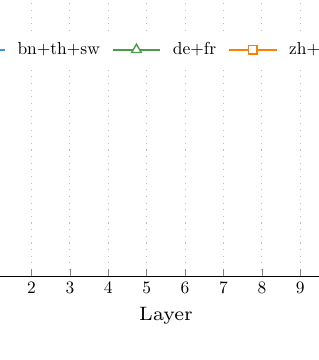
\begin{tikzpicture}
%%%%%%%%%%%%%%%%%%%%%%%%%%%%%%%%%%%%%%%%%%  
\useasboundingbox (13em,-1em) rectangle (3.5em,10em);
%%%%%%%%%%%%%%%%%%%%%%%%%%%%%%%%%%%%%%%%%%%%%%
\begin{axis}[
    global scale = 0.63,
    at={(1em,1em)},
    xtick pos=left,
    axis y line*=left,
    bar width=0.2cm,
    ymin=0, ymax=0.05,
    ytick={0,0.005,0.01,0.015,0.02,0.025,0.03,0.035,0.04,0.045,0.05},
    xtick={0,1,2,3,4,5,6,7,8,9,10},
    xticklabels={1,2,3,4,5,6,7,8,9,10},
    yticklabels={0,0.005,0.010,0.015,0.020,0.025,0.030,0.035,0.040,0.045,0.050},
    ylabel style={align=center},
    xtick=data,
    xticklabel style={
        inner sep=0pt,
        anchor=north,
        rotate=0,
        yshift=-3pt
    },
    yticklabel style={
        /pgf/number format/fixed,
        /pgf/number format/fixed zerofill,
        /pgf/number format/precision=2,
        rotate=0,
        scaled y ticks=false
    }
]              
    \addplot[sharp plot,ured,smooth,thick,line width=0.5pt,mark=*,mark size=1.4pt,thick,mark options={fill=ured,draw=ured,line width=0.5pt}] 
    plot coordinates {
        (1,0.0494) (2,0.0386) (3,0.0241)
        (4,0.0271) (5,0.0326) (6,0.0278)
        (7,0.0176) (8,0.0093) (9,0.0032)
        (10,0.0044)
    };\label{B1}                
\end{axis}
\begin{axis}[
    global scale = 0.63,
    at={(1em,1em)},
    legend entries={bn+th+sw,de+fr,zh+ru+es+ja},
    ymajorgrids=true,
    xmajorgrids=true,
    legend style={
        draw=none,
        line width=1pt,
        at={(10.5em,12.5em)},
        column sep=3pt,
        yshift=-5pt,
        anchor=south
    },
    axis y line*=right,
    xticklabels={},
    ymin=0.5, ymax=0.95,
    ytick={0.5,0.55,0.6,0.65,0.7,0.75,0.8,0.85,0.9,0.95},
    yticklabels={0.50,0.55,0.60,0.65,0.70,0.75,0.80,0.85,0.90,0.95},
    yticklabel style={
        /pgf/number format/fixed,
        /pgf/number format/fixed zerofill,
        /pgf/number format/precision=2,
        rotate=0
    }
]
    \addplot[sharp plot,ublue,smooth,thick,line width=0.5pt,mark=pentagon*,mark size=2pt,thick,mark options={fill=white,draw=ublue,line width=0.5pt}] 
    plot coordinates{
        (1,0.607)(2,0.595) (3,0.593)
        (4,0.609) (5,0.618) (6,0.627)
        (7,0.666) (8,0.694) (9,0.717)
        (10,0.728)
    };
    \addplot[sharp plot,udark,smooth,thick,line width=0.5pt,mark=triangle*,mark size=2pt,thick,mark options={fill=white,draw=udark,line width=0.5pt}] 
    plot coordinates {
        (1,0.656)(2,0.667) (3,0.672)
        (4,0.725) (5,0.788) (6,0.815)
        (7,0.850) (8,0.879) (9,0.892)
        (10,0.896)
    };
    \addplot[sharp plot,orange,smooth,thick,line width=0.5pt,mark=square*,mark size=1.6pt,thick,mark options={fill=white,draw=orange,line width=0.5pt}] 
    plot coordinates {
        (1,0.66)(2,0.648) (3,0.661)
        (4,0.698) (5,0.74) (6,0.769)
        (7,0.808) (8,0.836) (9,0.852)
        (10,0.856)
    };
\end{axis}
\node at (8.5em,-0.4em){\scriptsize Layer};

\node [rotate=90] at(-1.3em,4.9em){\scriptsize Mean Square Deviation};
\node [rotate=270] at(18.2em,5em){\scriptsize Overlap Ratio};
\end{tikzpicture}

\end{document}